\documentclass[12pt]{article}
\usepackage{fullpage,enumitem,amsmath,amssymb,graphicx}
\usepackage{listings} % This is a package for including code in your solution.
\usepackage{graphicx} % This is a package for including graphics in your solution.


\begin{document}

\begin{center}
{\Large CS168 Spring Assignment [1]}
\newline

\begin{tabular}{rll}
SUNet ID(s): & yyzhu & yd322 \\
Name(s): & Yueyao Zhu & Yang Du \\
Collaborators: & none
\end{tabular}
\end{center}

By turning in this assignment, I agree by the Stanford honor code and declare
that all of this is my own work.

\section*{Part 1}

\begin{enumerate}[label=(\alph*)]
  \item (See code \textbf{simu.py})
  \item (See \textbf{Figure~\ref{fig:plot}})
	\item (Answer to c)
\end{enumerate}

\begin{figure}[h]
	\centering
	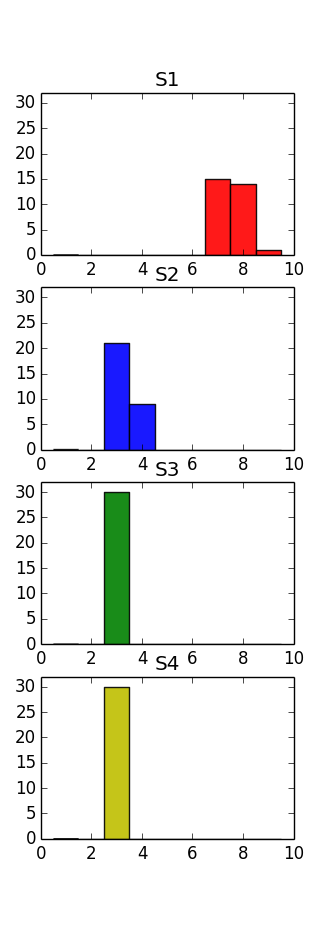
\includegraphics[width=0.4\textwidth]{figure_1.png}
	\caption{Histogram for $X$}
	\label{fig:plot}
\end{figure}

\end{document}